\section{Chain B -- CSV Loader (runs once at deploy)}

Loads \texttt{challenge3.csv} into the global context at deploy time so
that downstream chains can look up rows by packet number without
re-reading the file.

\begin{figure}[h]
    \centering
    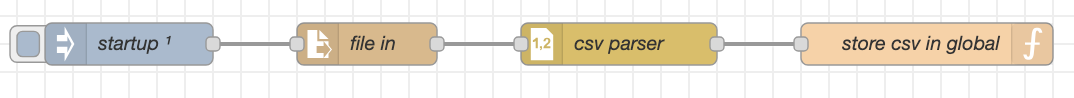
\includegraphics[width=0.85\linewidth]{images/flow_chain_b.png}
    \caption{Chain B -- CSV loader.}
\end{figure}

\begin{description}
    \item[startup (\emph{once on deploy})] fires a single message
        100\,ms after deploy.
    \item[file in] reads the entire \texttt{challenge3.csv} as a UTF-8
        string.
    \item[csv parser] converts the string into an array of row objects
        keyed by the column headers.
    \item[function \emph{store csv in global}] indexes the array by
        \texttt{Packet Number} and stores the resulting dictionary in
        \verb|global.challengeCsv|, providing $O(1)$ lookups.
        \begin{lstlisting}[caption={Store CSV in global}]
        const rows = msg.payload;
        const byPacketNum = {};
        for (const r of rows) {
            byPacketNum[r["Packet Number"]] = r;
        }
        global.set('challengeCsv', byPacketNum);
        node.warn(`Loaded ${rows.length} rows from challenge3.csv`);
        return null;
        \end{lstlisting}
\end{description}